
\chapter{TINJAUAN PUSTAKA}


\section{Landasan Teori}

\subsection{Citra Digital}
Citra digital dapat didefinisikan sebagai fungsi f(x,y) berukuran M baris dan N kolom, dengan x dan y adalah kordinat spasial, dan amplitudo f di titik kordinat (x,y) dinamakan intensitas atau tingkat keabuan dari citra pada citra tersebut \thecite{book:darma}. Pada umumnya warna dasar dalam citra RGB menggunakan penyimpanan 8 bit untuk menyimpan data warna, yang berarti setiap warna mempunyai gradasi sebanyak 255 warna . Dewasa ini, citra digital dapat menggunakan 16 bit untuk menyimpan data warna dasarnya, hal ini menyebabkan semakin banyak gradasi warnanya sehingga citra yang dihasilkan memiliki tingkat warna yang jauh lebih banyak. Namun tentu saja hal ini mengakibatkan ukuran file citra digital yang dihasilkan juga menjadi semakin besar walaupun dengan resolusi yang sama. Berdasarkan jenis warnanya citra digital dibagi menjadi 3 jenis:

\begin{enumerate} [label=\textbf{\alph*.}]
    \item \textbf{Citra Biner (monokrom)} \\ 
    Banyaknya dua warna, yaitu hitam dan putih. Warna hitam direpresentasikan dengan 1 dan warna putih direpresentasikan dengan 0. Dibutuhkan 1 bit di memori untuk menyimpan warna ini. Contoh citra biner dapat dilihat pada gambar ~\ref{fig:jenis-citra}(a).
    \item \textbf{Citra Grayscale} \\ 
    Banyaknya warna tergantung pada jumlah bit yang disediakan di memori untuk menampung kebutuhan warna ini. Citra 2 bit mewakili 4 warna, citra 3 bit mewakili 8 warna, dan seterusnya. Semakin besar jumlah bit warna yang disediakan di memori, semakin halus gradasi warna yang terbentuk. Pada umumnya citra digital grayscale menggunakan 8 bit memori dengan derajat keabuan dari 0 sampai 255. Contoh citra grayscale dapat dilihat pada gambar ~\ref{fig:jenis-citra}(b).
    \item \textbf{Citra Warna} \\ 
    Setiap piksel pada citra warna mewakili warna yang merupakan kombinasi dari tiga warna dasar (RG8 = Red Green Blue). Setiap warna dasar menggunakan penyimpanan 8 bit, yang berarti setiap warna mempunyai gradasi sebanyak 255 warna. Berarti setiap piksel mempunyai kombinasi warna sebanyak 255 x 255 x 255 =16 juta warna lebih. Dibutuhkan 3x8 = 24 bit di memori untuk menyimpan sebuah data warna ini. Contoh citra warna dapat dilihat pada gambar ~\ref{fig:jenis-citra}(c).
\end{enumerate}

\begin{afigure}
    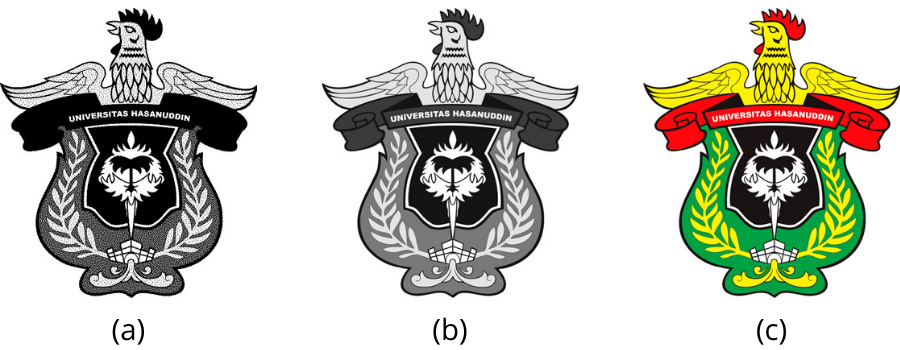
\includegraphics[width=0.85\textwidth, center]{images/jenis-jenis-citra.png}
    \caption{(a) Contoh citra biner, (b) contoh citra grayscale, (c) contoh citra warna.}
    \label{fig:jenis-citra}
\end{afigure}


\subsection{Pengolahan Citra Digital}
Pengolahan citra digital merupakan proses mengolah piksel-piksel di dalam citra digital untuk tujuan tertentu. Berdasarkan tingkat pemrosesannya pengolahan citra digital dikelompokkan menjadi tiga kategori, yaitu: \textit{low-level}, \textit{mid-level} dan pemrosesan \textit{high-level}. Pemrosesan \textit{low-level} dilakukan dengan operasi primitif seperti \textit{image preprocessing} untuk mengurangi derau (\textit{noise}), memperbaiki kontras citra dan mempertajam citra (\textit{sharpening}). Karakteristik dari pemrosesan \textit{low-level} yaitu keluaran atau hasil dari pemrosesannya berupa citra digital. Pemrosesan \textit{mid-level} melibatkan tugas-tugas seperti segmentasi (mempartisi gambar menjadi beberapa bagian atau objek), deskripsi objek untuk dilakukan pemrosesan lanjutan, dan klasifikasi objek dalam citra digital. Karakteristik dari pemrosesan \textit{mid-level} yaitu keluaran atau hasilnya berupa atribut atau fitur seperti, kontur, tepi, atau objek yang terdapat dalam citra tersebut. Pemrosesan \textit{high-level} merupakan proses tingkat lanjut dari dua proses sebelumnya, dilakukan untuk mendapat informasi lebih yang terkandung dalam citra \thecite{book:gonzalez}.

\subsection{Filter Spasial}
Konsep filter spasial pada pengolahan citra digital berasal dari penerapan transformasi Fourier untuk pemrosesan sinyal pada domain frekuensi. Istilah filter spasial ini digunakan untuk membedakan proses ini dengan filter pada domain frequensi. Proses filter dilakukan dengan cara menggeser filter kernel dari titik ke titik dalam citra digital. Istilah \textit{mask}, \textit{kernel}, \textit{template}, dan \textit{window} merupakan isitilah yang sama dan sering digunakan dalam pengolahan citra digital \thecite{book:gonzalez}. Dalam penelitian ini penulis menggunakan istilah kernel untuk istilah tersebut.


% Rumusnya
% rumusnya bisa dilihat pada \ref{eq:conv}
% Perbedaan Filter Linear dan Non Linear
Proses filter dalam pengolahan citra digital dilakukan dengan memanipulasi sebuah citra menggunakan kernel untuk menghasilkan citra yang baru, sehingga dengan kernel yang berbeda maka citra hasil yang didapat juga akan berbeda. 

\subsubsection{Operator Linear dan Non-linear}
Didefinisikan H sebuah operator dengan input dan output adalah citra digital. H dikatakan operator linear jika untuk untuk sembarang gambar \textit{f} dan \textit{g}, dan untuk sembarang skalar a dan b berkalu,
\begin{equation}
    \label{eq:linearity-operator}
    H(af + bg) = aH(f) + bH(g)
\end{equation}

Dengan kata lain hasil dari operator linear dengan jumlahan dua buah citra (yang telah dikali dengan konstanta a dan b) identik dengan hasil operator linear pada masing-masing gambar, dikali dengan konstanta yang sama, kemudian hasilnya dijumlahkan. Sebagai contoh, sebuah operator dengan fungsi yang menjumlahkan K citra adalah operator linear. Operator yang menghitung nilai absolut dari perbedaan dua gambar adalah tidak linear. Operator yang tidak memenuhi persamaan (\ref{eq:linearity-operator}) dikatakan non-linear \thecite{book:gonzalez}.

\subsection{Konvolusi}
Konsep filter spasial linear mirip seperti konsep konvolusi pada domain frekuensi, dengan alasan tersebut filter spasial linear biasa disebut juga konvolusi sebuah kernel dengan citra digital \thecite{book:gonzalez}. 

% Rumus konvolusi pada citra digital dapat dilihat pada persamaan (\ref{eq:conv}). K merupakan kernel yang digunakan dalam konvolusi, kemudian I merupakan citra yang akan dikonvolusi. 
% \begin{equation}
%     \label{eq:conv}
%     S(x,y) = (I * K)(x,y) = \sum_{i}^{} \sum_{j}^{} I(i,j)K(x-i, y-j)
% \end{equation}
% Keterangan: \\
%     \hspace{1cm} S(x,y) = fungsi \\
%     \hspace{1cm}  I = Citra yang dikonvolusi \\
%     \hspace{1cm} K = kernel \\
%     \hspace{1cm} x,y = pixel citra \\
%     \hspace{1cm} m,n = pixel kernel \\


Konvolusi pada fungsi f(x) dan g(x) didefinisikan sebagi berikut:
\begin{equation}
    \label{eq:conv1}
    \begin{split}
        h(x) = f(x) * g(x) = \int_{-\infty}^{\infty} f(a)g(x-a) da
    \end{split}
\end{equation}
dimana tanda * menyatakan operator konvolusi, dan peubah a adalah peubah bantu. Untuk fungsi diskrit, konvolusi didefinisikan sebagai:
\begin{equation}
    \label{eq:conv2}
    \begin{split}
         h(x) = f(x) * g(x) = \sum_{a=-\infty}^{\infty} f(a)g(x-a)
    \end{split}
\end{equation}

Pada operasi konvolusi diatas, g(x) disebut kernel konvolusi atau filter kernel. Kernel g(x) dioperasikan secara bergeser pada sinyal masukan f(x). Jumlah perkalian kedua fungsi pada setiap titik merupakan hasil konvolusi yang dinyatakan dengan keluaran h(x).


\subsection{Video Streaming}
Video stream dapat dipandang sebagai serangkaian citra digital berturut-turut \thecite{thesis:jin}. Berbeda dengan format video lainya, video stream ini tidak disimpan pada media penyimpanan sebagai file video melainkan langsung disalurkan setiap framenya dari sumber (source) ke penerima, dalam hal ini FPGA.  Dengan menganggap Video stream adalah kumpulan citra digital (frame) maka dapat dilakukan metode pengolahan seperti pada citra digital, termasuk filter spasial. 

\subsection{Frame Per Second (FPS)}


\subsection{FPGA}
Field Programmable Gate Arrays atau FPGA adalah perangkat semikonduktor yang berbasis \textit{matriks configurable logic block} (CLBs) yang terhubung melalui interkoneksi yang dapat diprogram. FPGA dapat diprogram ulang ke aplikasi atau fungsi yang diinginkan setelah \textit{manufacturing}. Fitur ini yang membedakan FPGA dengan \textit{Application Specific Integrated Circuits} (ASICs), yang dibuat khusus untuk tugas tertentu saja \thecite{XILINX}.

Sebuah \textit{microprocessor} menerima instruksi berupa kode 1 atau 0, kode-kode ini selanjutnya diinterpretasikan oleh komputer untuk menjalankan perintah yang diberikan. \textit{Microprocessor} ini membutuhkan intruksi berupa kode secara terus menerus untuk menjalankan fungsinya. Sedangkan pada FPGA hanya dibutuhkan sekali konfigurasi \textit{chip} setiap kali dinyalakan. Membuat atau mengunduh \textit{bitstream} yang menentukan fungsi logika dilakukan oleh \textit{logic elements} (LEs), sebuah sirkuit dapat dibuat dengan mengabungkan beberapa LEs menjadi satu kesatuan. Setelah \textit{bitstream} dipasang, FPGA tidak perlu lagi membaca instruksi berupa 1 dan 0, berbeda dengan \textit{microprocessor} yang selalu membutuhkan instruksi \thecite{pdf:cheung}. Secara tradisional, untuk membuat sebuah desain FPGA, aplikasi dideskripsikan menggunakan Hardware Description Language (HDL) seperti Verilog atau VHDL sehingga menghasilkan sebuah bitstream FPGA. 

\begin{afigure}
    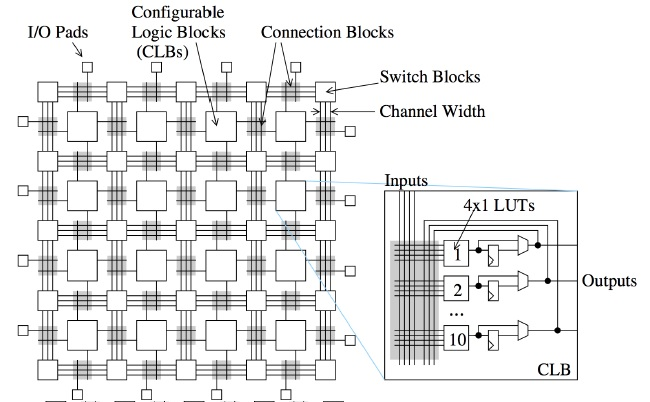
\includegraphics[width=12cm, center]{images/fpga-structure.jpeg}
    \caption{Struktur FPGA.}
    \label{fig:fpga-structure}
\end{afigure}

Pada FPGA terdahulu tidak terdapat processor (CPU) untuk menjalankan software apapun, sehingga ketika ingin mengimplementasikan aplikasi haruslah merancang sirkuit dari awal, seperti mengonfigurasi FPGA sesederhana gerbang logika OR atau serumit multi-core processor \thecite{site:biswas}. Dewasa ini telah dikembangkan \textit{FPGA Develepment Board} atau biasa disebut juga \textit{FPGA Board} yaitu teknologi FPGA yang dirangkai dalam sebuah \textit{board} dan dilengkapi dengan \textit{microprocessor} dan beberapa interface \textit{IO} untuk menjankan tugas tertenu. Umumnya FPGA Board telah dilengkapi dengan interface untuk mengakses dan menerapkan desain sirkuitnya. Xilinx, Altera dan Intel adalah produsen FPGA Board yang terkenal. FPGA Board yang digunakan dalam penelitian ini yaitu Xilinx PYNQ-Z2 dengan Jupyter Notebook sebagai interface untuk mengakses dan menjalankan program pada penelitian ini.

\begin{afigure}
    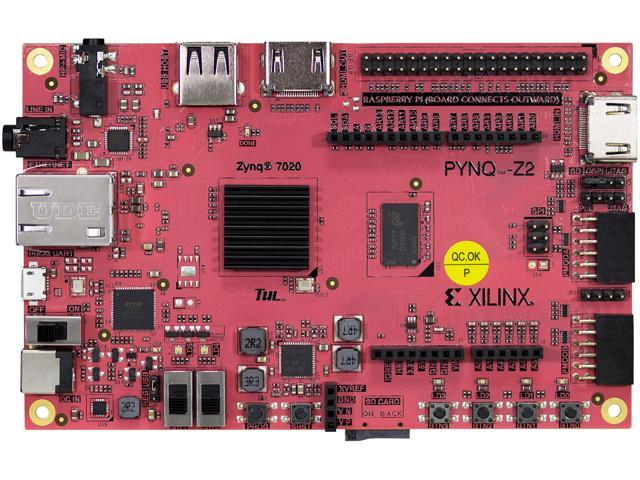
\includegraphics[width=6cm, center]{images/pynq-z2.jpeg}
    \caption{FPGA Board Xilinx PYNQ-Z2.}
    \label{fig:pynq-z2}
\end{afigure}

% perlu atau tidak?
% Jupyter juga?

% \subsection{Tepi Citra}
% Suatu titik (x, y) pada citra digital dikatakan sebagai tepi apabila perubahan nilai intensitas derajat keabuan yang mendadak (besar) dalam jarang yang berdekatan. Tepi biasanya terdapat pada batas andara dua daereah yang berbeda pada suatu citra. Tepi pada citra dapat merepresentasikan objek-objek yang terkandung dalam citra tersebut, bentuk dan ukurannya atau terkadang juga informasi tentang teksturnya.

% Tepi citra dapat dilihat melalui perubahan intensitas pixel pada suatu area. Berdasarkan perbedaan perubahan intensitas tersebut, tepi dapat dibagi menjadi 4 jenis yaitu tepi steep, ramp, line dan step-line \thecite{book:darma}.

% \begin{enumerate} [label=\textbf{\alph*.}]
%     \item \textbf{Steep}, tepi jenis \textit{step} merupakan tepi citra yang berbentuk dari perubahan intensitas nilai pixel secara signifikan dari tinggi ke rendah ataupun sebaliknya.
%     \item \textbf{Ramp}, tepi jenis ini terbentuk dari perubahan intensitas nilai pixel secara perlahan. Perubahan secara perlahan dapat dilihat pada bentuk kurva yang semakin tinggi dengan perubahan kontinu.
%     \item \textbf{Line}, tepi jenis ini ditandai dengan perubahan intensitas nilai pixel secara drastis dari rendah-tinggi-rendah atau sebaliknya.
%     \item \textbf{Step-Line}, tepi \textit{step-line} merupakan gabungan dari tepi jenis step dan line. Tepi jenis ini ditandai dengan peningkatan intensitas yang tajam dalam interval tertentu dan kemudian ditandai dengan penurunan yang tidak signifikan, sehingga perubahan intensitas nilai pixel selanjutnya berlangsung stabil.
% \end{enumerate}

% Tambahkan gambar 

% halaman 201
% https://books.google.co.id/books?hl=en&lr=&id=NectMutqXJAC&oi=fnd&pg=PR4&dq=buku+pengolahan+citra+digital&ots=C2oB2TDTo4&sig=UnkxuezGlrECiOZBepXOMa__gEY&redir_esc=y#v=onepage&q=buku%20pengolahan%20citra%20digital&f=false


% \subsection{Deteksi Tepi}
% Deteksi tepi merupakan salah satu metode dalam pemrosesan cira digital untuk deteksi fitur dan ekstraksi dengan mengidentifikasi titik-titik (pixel) dalam citra yang mengalami perubahan tingkat keabuan secara derastis dan mengalami diskontinu. Salah satu tujuan deteksi tepi yaitu untuk mengurangi jumlah data secara signifikan dalam suatu gambar dan mempertahankan sifat strukturalnya untuk pemrosesan citra lebih lanjut. \thecite{desi_herawati}.

% Berbagai macam metode deteksi dapat digunakan untuk mendeteksi tepi pada citra. Setiap teknik memiliki keunggulan dan karakteristiknya masing-masing. Suatu teknik deteksi tepi mungkin dapat bekerja sangat baik dalam suatu aplikasi tertentu namun sebaliknya belum tentu dapat berjalan secara maksimal pada aplikasi lainnya.

% Terdapat berbagai operator deteksi tepi yang telah dikembangkan berdasarkan turunan pertama (first order derrivate), di antaranya operator Robert, operator Sobel, operator Prewitt, operator Krisch, dan operator Canny. Konsep dasar dari deteksi tepi dengan turunan pertama adalah dengan memanfaatkan perbedaan nilai suatu pixel dengan pixel tetangganya. 
% operator turunan kedua, dan seterusnya


\section{Penelitian Terkait}
\subsection{Spatial Filtering Based Boundary Extraction in Underwater Images for Pipeline Detection: FPGA Implementation}
Pipa bawah air diletakkan di dasar laut untuk tujuan pengangkutan minyak bumi dan gas menyebrangi lautan. Pipa perlu terus dipantau untuk menghindari gangguan dalam proses transportasi. Gambar dasar laut dapat diperoleh dengan menggunakan kamera dan dengan memproses gambar yang diperoleh dapat membantu dalam mendeteksi pipa. Penelitian ini membahas tentang metode pemrosesan citra untuk deteksi pipa bawah laut dari gambar bawah laut yang diambil oleh kendaraan bawah laut yang dapat digunakan sebagai langkah awal untuk melacak saluran pipa. Implementasinya berhasil dilakukan pada Field Programmable Gate Array (FPGA) berbasis development board
\thecite{soa:alex-raj}.

\subsection{FPGA Implementation of Spatial Filtering techniques for 2D Images}
Berbagai teknik filter telah menjadi inti dari pemrosesan citra sejak awal teknik peningkatan citra (\textit{image enhancement}). Filter spasial domain pada pemrosesan citra digital digunakan dalam banyak kepentingan seperti mempertajam citra, menghaluskan citra, menghilangkan derau dan sebagainya. Fleksibilitas dari metode filter spasial sering dibandingkan dengan domain transformasi karena dapat digunakan untuk filter linear dan filter non-linear. Penghalusan citra dilakukan dengan langsung memanipulasi nilai intensitas dari citra asli dengan sebuah kernel filter. Hasilnya yaitu berkurangnya detail kecil dan derau pada citra. Penelitian ini tentang penerapan berbagai macam operator filter spasial. Hasilnya didasarkan pada konsumsi perangkat keras, kecepatan desain masing-masing arsitektur. Ukuran kualitas citra didapat dengan membandingkan output dari Matlab dan output dari Xilinx FPGA dan dengan menghitung MSE \thecite{soa:sushant}.

\subsection{Features of Image Spatial Filters Implementation on FPGA}
Penelitian ini menyajikan fitur-fitur implementasi filter spasial pada citra dengan Programmable Logic Integrated Circuits (FPGA). Solusi yang disajikan memungkinkan untuk membuat arsitektur kristal dengan performa tinggi untuk algoritma filter spasial. Hasilnya menunjukan kelebihan menggunakan \textit{programmable logic} dalam tugas pemrosesan gambar \thecite{soa:dmitry}.

\subsection{An FPGA-Oriented Algorithm for Real-Time Filtering of Poisson Noise in Video Streams, with Application to X-Ray Fluoroscopy}
Pada penelitian ini dibahas tentang algoritma baru untuk \textit{real-time filtering} pada video yang rusak karena \textit{poison noise}. Algorima yang disajikan efektif dalam penanganan derau, dan ini secara ideal cocok dengan implementasi hardware, dan dapat diimplementasikan pada FPGA kecil yang memiliki hardware resource yang terbatas. Pada penelitian ini penerapan algoritma menggukanan hasil X-ray fluoroscopy sebagai studi kasus. Hasil implementasi menggunakan yang StratixIV FPGA menunjukkan bahwa sistem hanya menggunakan, paling banyak, 22\% dari sumber daya perangkat, dalam im 
\thecite{soa:castellano}

\subsection{A real-time video denoising algorithm with FPGA implementation for Poisson-Gaussian noise}
\thecite{soa:xin}
